%!TEXTS-program = xelatex
%!TEX encoding = UTF-8 Unicode
\documentclass[a4paper, 11pt]{article}

%%%%%% 导入包 %%%%%%
\usepackage{xeCJK}
\usepackage{graphicx}
\usepackage{subfigure}
\usepackage[unicode]{hyperref}
\usepackage{xcolor}
\usepackage{cite}
\usepackage{indentfirst}
\usepackage{amsmath}
\usepackage{amssymb}
\usepackage{url}
\usepackage{algorithm}
\usepackage{algorithmic}
\usepackage{enumerate}
\usepackage{float}


%%%%%% 设置字号 %%%%%%
\newcommand{\chuhao}{\fontsize{42pt}{\baselineskip}\selectfont}
\newcommand{\xiaochuhao}{\fontsize{36pt}{\baselineskip}\selectfont}
\newcommand{\yihao}{\fontsize{28pt}{\baselineskip}\selectfont}
\newcommand{\erhao}{\fontsize{21pt}{\baselineskip}\selectfont}
\newcommand{\xiaoerhao}{\fontsize{18pt}{\baselineskip}\selectfont}
\newcommand{\sanhao}{\fontsize{15.75pt}{\baselineskip}\selectfont}
\newcommand{\sihao}{\fontsize{14pt}{\baselineskip}\selectfont}
\newcommand{\xiaosihao}{\fontsize{12pt}{\baselineskip}\selectfont}
\newcommand{\wuhao}{\fontsize{10.5pt}{\baselineskip}\selectfont}
\newcommand{\xiaowuhao}{\fontsize{9pt}{\baselineskip}\selectfont}
\newcommand{\liuhao}{\fontsize{7.875pt}{\baselineskip}\selectfont}
\newcommand{\qihao}{\fontsize{5.25pt}{\baselineskip}\selectfont}

%%% 英文相关字体属性 %%%%
% \usepackage{fontspec,xltxtra,xunicode}
% \defaultfontfeatures{Mapping=tex-text}
% \setromanfont[Mapping=tex-text]{Hoefler Text}
% \setsansfont[Scale=MatchLowercase,Mapping=tex-text]{Gill Sans}
% \setmonofont[Scale=MatchLowercase]{Andale Mono}

%%%% 设置 font 属性 %%%%
\setCJKmainfont[BoldFont ={STXihei},ItalicFont ={STKaiti}]{STFangsong}%{STSong}  %设置中文正体字体,BoldFont设置粗体和斜体样式对应的字体
\setCJKsansfont{STXihei}%设置无衬线样式对应字体
\setCJKmonofont{STFangsong} %设置有衬线样式对应字体
\punctstyle{hangmobanjiao} %行末半角式:所有标点占一个汉字宽度,行首行末对齐

%%%% 设置 section 属性 %%%%
\makeatletter
\renewcommand\section{\@startsection{section}{1}{\z@}%
{-1.5ex \@plus -.5ex \@minus -.2ex}%
{.5ex \@plus .1ex}%
{\normalfont\sihao\CJKfamily{hei}}}
\makeatother

%%%% 设置 subsection 属性 %%%%
\makeatletter
\renewcommand\subsection{\@startsection{subsection}{1}{\z@}%
{-1.25ex \@plus -.5ex \@minus -.2ex}%
{.4ex \@plus .1ex}%
{\normalfont\xiaosihao\CJKfamily{hei}}}
\makeatother

%%%% 设置 subsubsection 属性 %%%%
\makeatletter
\renewcommand\subsubsection{\@startsection{subsubsection}{1}{\z@}%
{-1ex \@plus -.5ex \@minus -.2ex}%
{.3ex \@plus .1ex}%
{\normalfont\xiaosihao\CJKfamily{hei}}}
\makeatother

%%%% 段落首行缩进两个字 %%%%
\makeatletter
\let\@afterindentfalse\@afterindenttrue
\@afterindenttrue
\makeatother
\setlength{\parindent}{2em}  %中文缩进两个汉字位


%%%% 下面的命令重定义页面边距,使其符合中文刊物习惯 %%%%
\addtolength{\topmargin}{-54pt}
\setlength{\oddsidemargin}{0.63cm}  % 3.17cm - 1 inch
\setlength{\evensidemargin}{\oddsidemargin}
\setlength{\textwidth}{14.66cm}
\setlength{\textheight}{24.00cm}    % 24.62

%%%% 下面的命令设置行间距与段落间距 %%%%
\linespread{1.4}
% \setlength{\parskip}{1ex}
\setlength{\parskip}{0.5\baselineskip}

%%%% 正文开始 %%%%
\begin{document}

%%%% 定理类环境的定义 %%%%
\newtheorem{example}{例}             % 整体编号
% \newtheorem{algorithm}{算法}
\newtheorem{theorem}{定理}[section]  % 按 section 编号
\newtheorem{definition}{定义}
\newtheorem{axiom}{公理}
\newtheorem{property}{性质}
\newtheorem{proposition}{命题}
\newtheorem{lemma}{引理}
\newtheorem{corollary}{推论}
\newtheorem{remark}{注解}
\newtheorem{condition}{条件}
\newtheorem{conclusion}{结论}
\newtheorem{assumption}{假设}

%%%% 重定义 %%%%
\renewcommand{\contentsname}{目录}  % 将Contents改为目录
\renewcommand{\abstractname}{摘要}  % 将Abstract改为摘要
\renewcommand{\refname}{参考文献}   % 将References改为参考文献
\renewcommand{\indexname}{索引}
\renewcommand{\figurename}{图}
\renewcommand{\tablename}{表}
\renewcommand{\appendixname}{附录}
%\renewcommand{\algorithm}{算法}
\newcommand{\upcite}[1]{\textsuperscript{\cite{#1}}}
\makeatletter
\@addtoreset{equation}{section}
\@addtoreset{figure}{section}
\makeatother
\renewcommand{\theequation}{\arabic{section}.\arabic{equation}}
\renewcommand{\thefigure}{\arabic{section}.\arabic{figure}}

\renewcommand{\algorithmicrequire}{\textbf{Input:}} % Use Input in the format of Algorithm
\renewcommand{\algorithmicensure}{\textbf{Output:}} % Use Output in the format of Algorithm

%%%% 定义标题格式,包括title,author,affiliation,email等 %%%%
\title{图像处理报告}
\author{王晗\footnote{电子邮件: hanwang.0501@gmail.com,学号: 2014141463191}\\[2ex]
\xiaosihao 四川大学吴玉章学院\\[2ex]
}
\date{2017年11月}


%%%% 以下部分是正文 %%%%
\maketitle

\tableofcontents
\newpage
\section{风格迁移}

风格迁移是指一张图片的艺术风格迁移到另一张图片上,艺术风格是什么以及如何定义一种艺术风格,每个人都有每个人的见解,有些东西大概艺术界也没明确的定义。如何要把一个图像的风格变成另一种风格更是难以定义的问题。

在神经网络之前,传统的图像风格迁移方法有一个共同的思路:分析某一种风格的图像,给那一种风格建立一个数学或者统计模型,再改变要做迁移的图像让它能更好的符合建立的模型。这样做出来效果还是不错的,比如下面的三张图中所示,但一个很大的缺点:一个程序基本只能做某一种风格或者某一个场景。因此基于传统风格迁移研究的实际应用非常有限。

随着深度学习的兴起,以及当代计算机计算能力的快速提高,人工智能算法逐渐走出实验室,投入了科研和商用的诸多领域的实际应用之中。2015年Gatys发表利用深度学习进行图像风格转移的论文\footnote{论文名:A neural algorithm of artistic style,论文地址:https://arxiv.org/pdf/1508.06576v2.pdf}。在这之前让程序模仿任意一张图片画画是没法想象的,也标志着风格转移研究进入了新的历史阶段\cite{history}。
\section{基于传统方法的风格迁移算法}

\subsection{基于Laplace金字塔算法}

图像金字塔是图像中多尺度表达的一种,最主要用于图像的分割,是一种以多分辨率来解释图像的有效但概念简单的结构。图像金字塔最初用于机器视觉和图像压缩,一幅图像的金字塔是一系列以金字塔形状排列的分辨率逐步降低,且来源于同一张原始图的图像集合。其通过梯次向下采样获得,直到达到某个终止条件才停止采样。金字塔的底部是待处理图像的高分辨率表示,而顶部是低分辨率的近似。我们将一层一层的图像比喻成金字塔,层级越高,则图像越小,分辨率越低。形象表示如图\ref{img:图像金字塔}所示。

\begin{figure}[H]
    \centering
    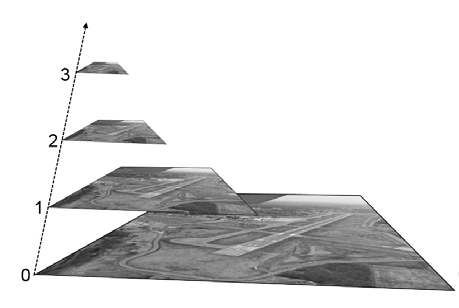
\includegraphics[width=2.00in,height=1.236in]{imgs/laplace.jpg}
    \label{img:图像金字塔}
    \caption{图像金字塔}
\end{figure}

算法主要利用了图像的频域信息,因为频域信息可以看做其中蕴含了该图像的风格。通过对图像的高频和低频进行操作变换,即可完成图像的风格迁移。使用的算法如算法\ref{alg:基于Laplace的风格迁移算法}所示:

\begin{algorithm}[H]
\caption{基于Laplace的风格迁移算法}  
\label{alg:基于Laplace的风格迁移算法}  
\begin{algorithmic}[1]
    \REQUIRE 源图像$ref\_img$,风格图像$src\_img$
    \ENSURE 融合后的目标图像$res\_img$
    \STATE 初始化 $res\_img=src\_img$
    \FOR  {each 通道$\in \{r,g,b\}$} 
    \STATE 分别利用$Laplace$金字塔得到风格图像和源图像的高频和低频部分
    \STATE 在给定的窗口大小中,分别得到风格图像和源图像的对比度
    \STATE $res\_img$[当前通道]低频部分等于参考图像和源图像低频部分频率最低的部分
    \STATE $res\_img$[当前通道]高频部分等于参考图像和源图像高频部分对比度最大的部分
    \STATE $res\_img$[当前通道]基于得到的高频和低频部分进行小波逆变换
    \ENDFOR 
\end{algorithmic}  
\end{algorithm}

\subsection{基于小波变换算法}
 众所周知,图像的傅里叶变换是将图像信号分解为各种不同频率的正弦波。同样,小波变换是将图像信号分解为由原始小波位移和缩放之后的一组小波。小波在图像处理里被称为图像显微镜,原因在于它的多分辨率分解能力可以将图片信息一层一层分解剥离开来。剥离的手段就是通过低通和高通滤波器。我们知道,图像的低频部分保存的是图像的轮廓信息,而高频保存的是图像的边缘和细节信息。同样的通过对图像的高频和低频进行操作,即可实现图像风格的迁移\cite{trad}。使用的算法如算法\ref{alg:基于小波变换的风格迁移算法}所示:
\begin{algorithm}[H]
\caption{基于小波变换的风格迁移算法}  
\label{alg:基于小波变换的风格迁移算法}  
\begin{algorithmic}[1]
    \REQUIRE 源图像$ref\_img$,风格图像$src\_img$
    \ENSURE 融合后的目标图像$res\_img$
    \STATE 初始化 $res\_img=src\_img$
    \FOR  {each 通道$\in \{r,g,b\}$} 
    \STATE 分别利用小波变换得到风格图像和源图像的高频和低频部分
    \STATE 分别计算风格图像和源图像的方差权重比
    \STATE $res\_img$[当前通道]低频部分等于参考图像和源图像按照方差权重比的叠加
    \STATE 在给定的窗口大小中,分别得到风格图像和源图像的对比度
    \STATE $res\_img$[当前通道]高频部分等于参考图像和源图像高频部分对比度最大的部分
    \STATE $res\_img$[当前通道]的低频和高频部分叠加
    \ENDFOR 
\end{algorithmic}  
\end{algorithm}


\subsection{实验结果}
对于彩色通道的图片,对RGB三个分别使用以上算法,得到三个通道的输出结果,再讲三个通道的结果拼成最后生成的RGB图像。结果如下图所示

\begin{figure}[H]
    \centering
    \subfigure[在R通道上的迁移结果]{
        \label{fig:subfig:r} %% label for first subfigure
        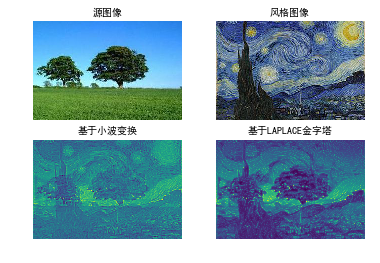
\includegraphics[width=2.5in]{imgs/r.png}}
    \hspace{0.1 in}
    \subfigure[在G通道上的迁移结果]{
        \label{fig:subfig:g} %% label for second subfigure
        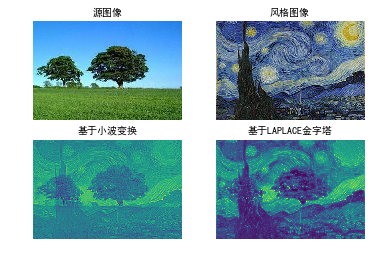
\includegraphics[width=2.5 in]{imgs/g.png}}
    \hspace{0.1in}
    \subfigure[在B通道上的迁移结果]{
        \label{fig:分别在RGB三通道上的迁移结果:b} %% label for second subfigure
        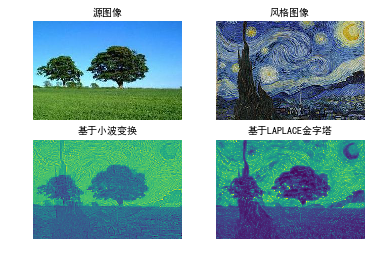
\includegraphics[width=2.5 in]{imgs/b.png}}
\caption{分别在RGB三通道上的迁移结果}
\label{fig:分别在RGB三通道上的迁移结果} %% label for entire figure
\end{figure}

在RGB通道上整体的显示结果:
\begin{figure}[H]
    \centering
    \label{fig:迁移} %% label for first subfigure
    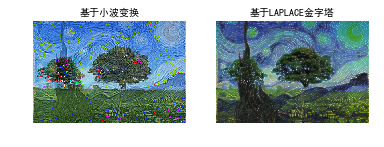
\includegraphics[width=4 in]{imgs/total.png}
    \caption{迁移结果}
    \label{fig:迁移结果}
\end{figure}

为了保持图像色彩风格的一致,使用了$reinhard$算法(算法\ref{alg:reinhard算法})来迁移图像的色彩风格\cite{reinhard}。
\begin{algorithm}[H]
\caption{$reinhard$算法}  
\label{alg:reinhard算法}  
\begin{algorithmic}[1]
    \REQUIRE 源图像$ref\_img$,风格图像$src\_img$
    \ENSURE 融合后的目标图像$res\_img$
    \STATE 将风格图像和源图像转换到LAB颜色空间下
    \STATE 计算风格图像和源图像的均值和标准差
    \STATE 为了得到目标图像,将风格图像的每个像素值,减去源图像的均值然后乘以风格图像和源图像标准差的比值,再加上风格图像的均值
    \STATE 目标图像转换到RGB空间
\end{algorithmic}  
\end{algorithm}

在进行基于$Laplace$金字塔算法和基于小波变换的算法前,先使用$reinhard$算法,结果如下
\begin{figure}[H]
    \centering
    \subfigure[用$reinhard$算法在R通道上的迁移结果]{
        \label{fig:用reinhard算法:r} %% label for first subfigure
        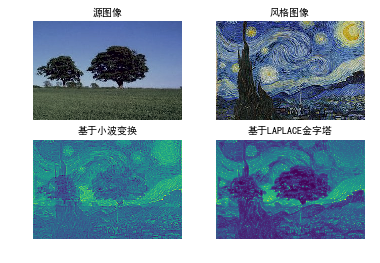
\includegraphics[width=2.5in]{imgs/reinhard_r.png}}
    \hspace{0.1 in}
    \subfigure[用$reinhard$算法在G通道上的迁移结果]{
        \label{fig:用reinhard算法:g} %% label for second subfigure
        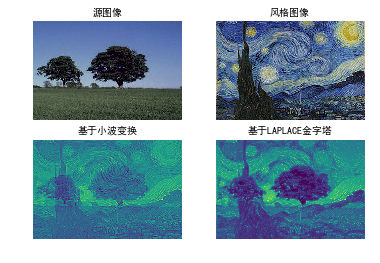
\includegraphics[width=2.5 in]{imgs/reinhard_g.png}}
    \hspace{0.1in}
    \subfigure[用$reinhard$算法在B通道上的迁移结果]{
        \label{fig:用reinhard算法:b} %% label for second subfigure
        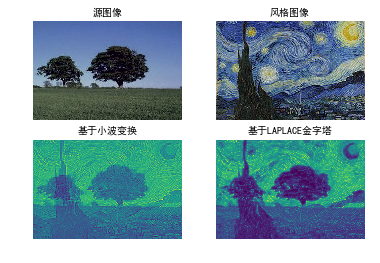
\includegraphics[width=2.5 in]{imgs/reinhard_b.png}}
\caption{用$reinhard$算法分别在RGB三通道上的迁移结果}
\label{fig:用$reinhard$算法分别在RGB三通道上的迁移结果} 
\end{figure}

在RGB通道上整体的显示结果:
\begin{figure}[H]
    \centering
    \label{fig:用reinhard算法迁移} %% label for first subfigure
    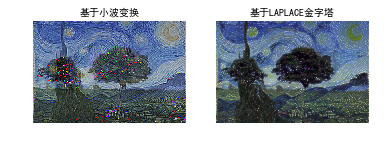
\includegraphics[width=4 in]{imgs/reinhard_total.png}
    \caption{用$reinhard$算法迁移结果}
    \label{fig:用reinhard算法迁移结果} %% label for entire figure
\end{figure}

\section{基于神经网络的风格迁移算法}

\subsection{神经网络概述}
要说明风格迁移算法的算法流程,就不得不先介绍一下算法的基础——卷积神经网络。普通的神经网络难以处理图像数据的根本原因就是如果把图像的每个像素都视作一个输入值,那么输入层一定十分庞大。按照一般神经网络每一层之间都进行全连接的结构,对于稍大的图片,建立其对应的神经网络将需要储存数量难以估计的参数数据,网络结构也会随着层数的增加变得非常庞大和复杂。而卷积神经网络却可以做到使用多层网络处理大型图像数据的同时,保持很小的参数数据量和计算量,这与卷积神经网络特殊的结构有关。
\begin{figure}[H]
\centering
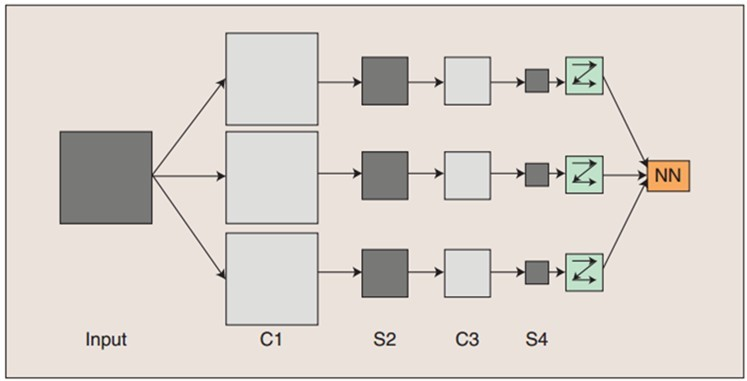
\includegraphics[width=3.00in,height=1.854in]{imgs/cnn_art.jpg}
\caption{典型的CNN结构}
\end{figure}
卷积神经网络的结构本就是来自于上世纪60年代对猫脑皮层的研究,卷积神经网络一开始就是一种仿生的神经网络。卷积神经网络的基本结构是两种特殊的隐含层——卷积层和池化层。卷积层与上一层的输入神经元节点不进行全连接,而是进行局部连接,并且同一个卷积网络(又称卷积核)中的所有神经元节点共享相同的权值参数。而池化层往往紧跟在卷积层的后面,池化层的作用就是直接减少神经元的数目,以下采样的方式直接简化上一卷积层的数据。这么一来,相比起普通的神经网络,卷积神经网络的参数数据和整体的神经节点数目都非常少。并且与此同时,卷积神经网络的局部链接、权值共享以及时间或空间亚采样这三种结构思想结合起来获得了某种程度的对于图像的位移、尺度、形变的不变性。

\subsection{原始风格迁移}
原始的风格迁移的速度是非常慢的。在GPU上,生成一张图片都需要10分钟左右,而如果只使用CPU而不使用GPU运行程序,甚至需要几个小时。这个时间还会随着图片尺寸的增大而迅速增大。这其中的原因在于,在原始的风格迁移过程中,把生成图片的过程当做一个“训练”的过程。每生成一张图片,都相当于要训练一次模型,这中间可能会迭代几百几千次,从头训练一个模型要比执行一个已经训练好的模型要费时太多。而这也正是原始的风格迁移速度缓慢的原因。

用于风格迁移算法的VGG网络一共使用了19层计算层,其中14层为卷积层,5层作为池化层。风格迁移算法的关键便在于使用VGG网络“分离”了输入图像的内容和风格。然后通过随机生成一个白噪音图像,根据得到的两幅图像的分别的内容和风格,不断迭代生成理想的图像。

在内容图片方面,由于卷积神经网络随着层数的增加会不断的进行下取样操作,所以越是在网络高层,网络内部存储的特征数据就越接近图片的全局结构,而相应的,图像的局部结构和像素信息就会不断丢失。换句话来说,网络越高层,因为单个节点对应的原图像的输入节点就越多,储存的图像信息就越抽象,但由于输入节点的信息进行了更多次的下取样,具体信息会渐渐消失。所以在网络高层获得图像特征数据,就可以视作图像的内容,由于此时图像的细节像素信息和局部结构信息已经丢失,我们就可以视作图片的风格数据已经被分离出去了。

而在风格图片方面,卷积神经网络本没有定义图像风格相关的数据。在这个算法中我们在每一个卷积层额外开辟一个空间来储存图像风格数据,而具体的图像风格数据则使用该层节点作为元素的格拉姆矩阵来得到。类似内容图片,风格也是在越高层越抽象。我们在高层提取的风格数据即可视作这个图像的风格数据\cite{nnmethod}。

最后生成图像部分,首先生成一个白噪音图像。定义两个损失方程:内容损失方程和风格损失方程:

内容损失方程:
\begin{equation}
L_{content}(\vec{p},\vec{x},l)=\frac{1}{2}\sum_{i,j}(F_{ij}^{l}-P_{ij}^{l})^2
\end{equation}

风格损失方程:
\begin{equation}
L_{style}(\vec{a},\vec{x})=\sum_{t=0}^{L}w_lE_l
\end{equation}

其中$F_{ij}^{l}$和$P_{ij}^{l}$分别是原图像和输出图像卷积神经网络中第$l$层第$i$个过滤器第$j$个位置神经元节点的激发值。而$E_l=\frac{1}{4N_l^2M_l^2}\sum_{ij}(G_{ij}^{l}-A_{ij}^{l})^2$是第$l$层造成的风格损失值。最后定义总损失方程:
\begin{equation}
L_{total}(\vec{p},\vec{a},\vec{x})=\alpha L_{content}(\vec{p},\vec{x})+\beta L_{style}(\vec{a},\vec{x})
\end{equation}
生成白噪音图像之后,通过对两个损失方程对$F_{ij}^{l}$求导数来进行梯度下降算法最小化总损失,并不断迭代,直至一定的迭代次数或者总损失足够的小。此时生成的图像即是同时拥有内容图片的内容和风格图片的风格的新图片。

\subsection{快速风格迁移}
\label{subsection:快速风格迁移}

快速风格转移很好的解决了原始风格迁移速度缓慢的问题\footnote{论文名:Perceptual Losses for Real-Time Style Transfer and Super-Resolution,论文地址:https://arxiv.org/pdf/1603.08155.pdf}。它不把生成图片当做一个“训练”的过程,而当成一个“执行”的过程。快速风格迁移的网络结构包含两个部分。一个是“生成网络”,一个是“损失网络。生成网络接收一个图片当做输入,然后输出也是一张图片(即风格迁移后的结果)。如下图,左侧是生成网络,右侧为损失网络:
\begin{figure}
\centering
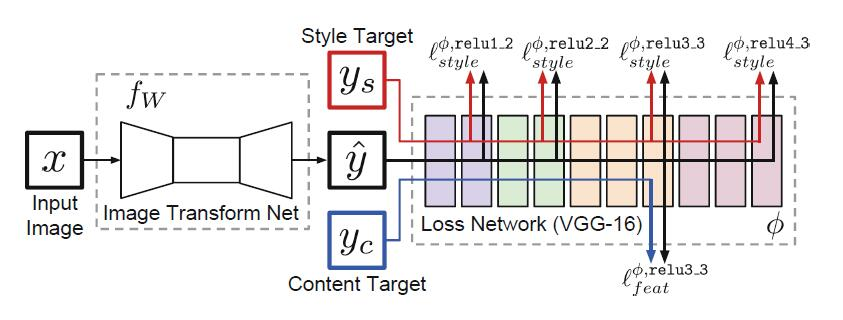
\includegraphics[width=5.00in,height=1.8 in]{imgs/fast_cnn_transfer.jpg}
\caption{快速风格迁移网络结构}
\end{figure}
在训练阶段中,首先选定一张风格图片。训练的目标是让生成网络可以有效生成图片,目标由损失网络定义。在执行阶段中,给定一张图片,将其输入生成网络,输出这张图片风格迁移后的结果。我们可以发现,在模型的“执行”阶段我们就可以完成风格图片的生成。

同样的,快速风格迁移方法使用了19层的VGG网络,同样定义了两个损失方程:特征重建损失方程和风格重建损失方程。

特征重建损失方程:
\begin{equation}
\ell^{\phi,j}_{feat}(\hat{y},y)=\frac{1}{C_jH_jW_j}\left \|\phi_j(\hat{y}-\phi_j(y))  \right \|^2_2
\end{equation}

其中,$\phi_j(x)$是网络$\phi$处理输入图像$x$的第$j$层的激活输出。$C_j\times H_j \times W_j$是特征图谱的大小。

风格重建损失方程:

\begin{equation}
\ell^{\phi,j}_{style}(\hat{y},y)=\left \|G^{\phi}_j(\hat{y})-G^{\phi}_j(y)  \right \|^2_F
\end{equation}

其中,$G^\phi_j(x)$为\emph{GRAM}矩阵。

在训练阶段,输入风格图像后,训练目标是最小化以上提到的两个损失方程加上$TV$正则项。
\begin{equation}
\hat{y}=arg\,\underset{y}{min}\lambda_c\ell^{\phi,j}_{feat}(y,y_c)+\lambda_s\ell^{\phi,j}_{style}(y,y_s)+\lambda_{TV}\ell_{TV}(y)
\end{equation}
然后通过梯度下降算法求出最优解,得到该风格图像的风格迁移网络。最后当训练后风格迁移网络后,输入目标图像,然后通过网络,生成的就是我们想要的有风格图像的特征的目标图像了。

\subsection{实验结果}

以下实验结果基于快速风格迁移算法\ref{subsection:快速风格迁移}。

\section{算法意义以及未来趋势}
风格迁移算法一经问世,便受到学术界的广泛关注和探讨。在2016年,Google提出的新论文\emph{A Learned Representation for Artistic Style\footnote{论文地址:https://arxiv.org/pdf/1610.07629.pdf}}中以该算法为基础,提出了新的风格混合算法。这个算法突破了原风格迁移算法只能迁移一个风格图片的风格的限制,其可以提取任意多的风格图片的风格,并根据输入权重任意混合得到的艺术风格,以全新的艺术风格绘制出新的图片。相比起只能做单个风格迁移的风格迁移算法,风格混合算法已经完全迈入艺术创作的领域当中了。

虽然并不能代表人工智能目前已经可以在艺术创作这个领域代替人类进行工作,但是其成功说明诸如艺术创造等涉及想象和艺术感知等人类高级思维的思考过程的领域不是完全不能进行数学建模和分析的。这说明一方面和其他领域无异,我们可以尝试在这些涉及高级思维过程的领域使用当前已经很成熟的人工智能算法,让计算机介入。另外一个方面,这些涉及高级思维过程的领域的工作也不是全部无章可循,计算机拟合的可能性是有的。

还有最为关键的,现在已有的研究结果已经证明,卷积神经网络得到图像特征的过程和生物形成视觉的过程有着惊人的类似——双方都是逐层从具体的光学数据渐渐得到图像的抽象信息。而此类算法的成功,为我们指明了一条可能可以通过人工智能算法从机器人视觉去理解人类创作各种艺术意象的过程,理解人类是如何感知艺术意象的道路。

\bibliographystyle{ieeetr}
\bibliography{image_style_report}

\end{document}
